\documentclass{standalone}
\usepackage{tikz}
\usetikzlibrary{patterns, positioning}


\begin{document}
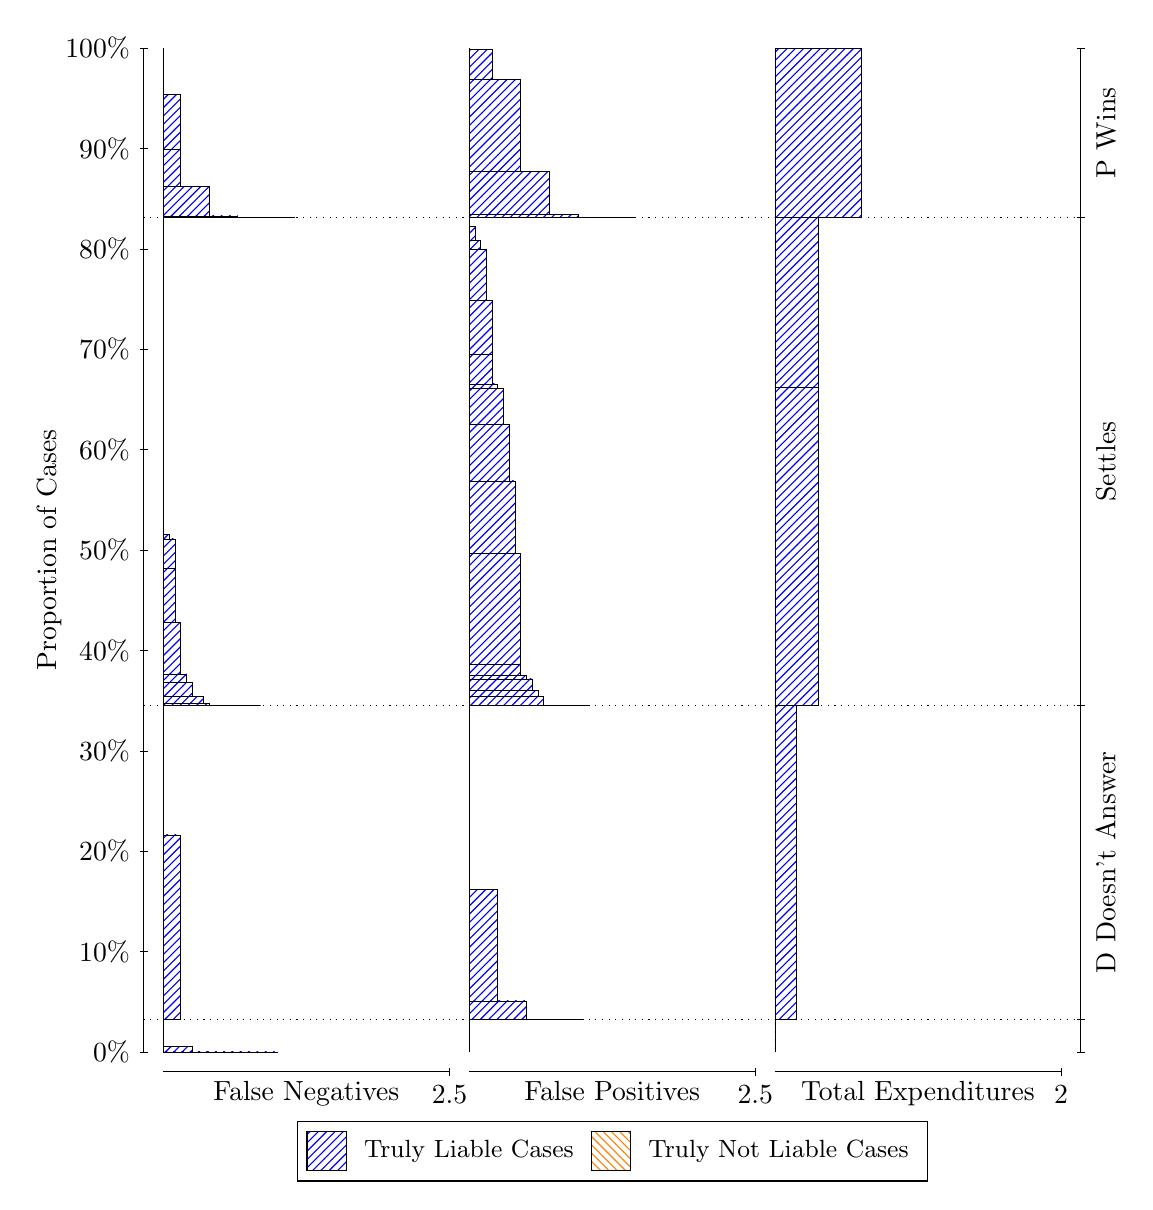
\begin{tikzpicture}
\draw[black, very thin] (1.5,1.75) -- (1.5,14.5);
\node[rotate=90, text=black, anchor=center] at (0.3, 8.125) {Proportion of Cases};
\draw[black, very thin] (1.45,1.75) -- (1.55,1.75);
\node[text=black, anchor=east] at (1.45, 1.75) {0\%};
\draw[black, very thin] (1.45,3.025) -- (1.55,3.025);
\node[text=black, anchor=east] at (1.45, 3.025) {10\%};
\draw[black, very thin] (1.45,4.3) -- (1.55,4.3);
\node[text=black, anchor=east] at (1.45, 4.3) {20\%};
\draw[black, very thin] (1.45,5.575) -- (1.55,5.575);
\node[text=black, anchor=east] at (1.45, 5.575) {30\%};
\draw[black, very thin] (1.45,6.85) -- (1.55,6.85);
\node[text=black, anchor=east] at (1.45, 6.85) {40\%};
\draw[black, very thin] (1.45,8.125) -- (1.55,8.125);
\node[text=black, anchor=east] at (1.45, 8.125) {50\%};
\draw[black, very thin] (1.45,9.4) -- (1.55,9.4);
\node[text=black, anchor=east] at (1.45, 9.4) {60\%};
\draw[black, very thin] (1.45,10.675) -- (1.55,10.675);
\node[text=black, anchor=east] at (1.45, 10.675) {70\%};
\draw[black, very thin] (1.45,11.95) -- (1.55,11.95);
\node[text=black, anchor=east] at (1.45, 11.95) {80\%};
\draw[black, very thin] (1.45,13.225) -- (1.55,13.225);
\node[text=black, anchor=east] at (1.45, 13.225) {90\%};
\draw[black, very thin] (1.45,14.5) -- (1.55,14.5);
\node[text=black, anchor=east] at (1.45, 14.5) {100\%};

\draw[black, very thin] (13.4,1.75) -- (13.4,14.5);
\draw[black, very thin] (13.35,1.75) -- (13.45,1.75);
\node[anchor=west] at (13.35, 1.75) {};
\draw[black, very thin] (13.35,2.1624) -- (13.45,2.1624);
\node[anchor=west] at (13.35, 2.1624) {};
\draw[black, very thin] (13.35,6.1553) -- (13.45,6.1553);
\node[anchor=west] at (13.35, 6.1553) {};
\draw[black, very thin] (13.35,12.345) -- (13.45,12.345);
\node[anchor=west] at (13.35, 12.345) {};
\draw[black, very thin] (13.35,14.5) -- (13.45,14.5);
\node[anchor=west] at (13.35, 14.5) {};

\draw[black, very thin, pattern color=blue, pattern=north east lines] (1.75,1.75) rectangle (3.2033,1.75);
\draw[black, very thin, pattern color=blue, pattern=north east lines] (1.75,1.75) rectangle (2.84,1.75);
\draw[black, very thin, pattern color=blue, pattern=north east lines] (1.75,1.75) rectangle (2.4767,1.7506);
\draw[black, very thin, pattern color=blue, pattern=north east lines] (1.75,1.7506) rectangle (2.1133,1.8175);
\draw[black, very thin, pattern color=orange, pattern=north west lines] (1.75,1.8175) rectangle (1.75,1.8175);
\draw[black, very thin, pattern color=blue, pattern=north east lines] (1.75,1.8175) rectangle (1.75,2.1624);
\draw[black, very thin, pattern color=blue, pattern=north east lines] (1.75,2.1624) rectangle (1.968,4.5073);
\draw[black, very thin, pattern color=orange, pattern=north west lines] (1.75,4.5073) rectangle (1.75,4.5073);
\draw[black, very thin, pattern color=blue, pattern=north east lines] (1.75,4.5073) rectangle (1.75,6.1553);
\draw[black, very thin, pattern color=blue, pattern=north east lines] (1.75,6.1553) rectangle (2.9853,6.1553);
\draw[black, very thin, pattern color=blue, pattern=north east lines] (1.75,6.1553) rectangle (2.84,6.1553);
\draw[black, very thin, pattern color=blue, pattern=north east lines] (1.75,6.1553) rectangle (2.6947,6.1553);
\draw[black, very thin, pattern color=blue, pattern=north east lines] (1.75,6.1553) rectangle (2.622,6.1554);
\draw[black, very thin, pattern color=blue, pattern=north east lines] (1.75,6.1554) rectangle (2.5493,6.1554);
\draw[black, very thin, pattern color=blue, pattern=north east lines] (1.75,6.1554) rectangle (2.4767,6.1554);
\draw[black, very thin, pattern color=blue, pattern=north east lines] (1.75,6.1554) rectangle (2.404,6.1556);
\draw[black, very thin, pattern color=blue, pattern=north east lines] (1.75,6.1556) rectangle (2.3313,6.1772);
\draw[black, very thin, pattern color=blue, pattern=north east lines] (1.75,6.1772) rectangle (2.2587,6.2647);
\draw[black, very thin, pattern color=blue, pattern=north east lines] (1.75,6.2647) rectangle (2.186,6.2651);
\draw[black, very thin, pattern color=blue, pattern=north east lines] (1.75,6.2651) rectangle (2.1133,6.4465);
\draw[black, very thin, pattern color=blue, pattern=north east lines] (1.75,6.4465) rectangle (2.0407,6.5507);
\draw[black, very thin, pattern color=blue, pattern=north east lines] (1.75,6.5507) rectangle (1.968,7.2078);
\draw[black, very thin, pattern color=blue, pattern=north east lines] (1.75,7.2078) rectangle (1.8953,7.8866);
\draw[black, very thin, pattern color=blue, pattern=north east lines] (1.75,7.8866) rectangle (1.8953,8.2665);
\draw[black, very thin, pattern color=blue, pattern=north east lines] (1.75,8.2665) rectangle (1.8227,8.3211);
\draw[black, very thin, pattern color=orange, pattern=north west lines] (1.75,8.3211) rectangle (1.75,8.3211);
\draw[black, very thin, pattern color=blue, pattern=north east lines] (1.75,8.3211) rectangle (1.75,12.345);
\draw[black, very thin, pattern color=blue, pattern=north east lines] (1.75,12.345) rectangle (3.4213,12.345);
\draw[black, very thin, pattern color=blue, pattern=north east lines] (1.75,12.345) rectangle (3.058,12.346);
\draw[black, very thin, pattern color=blue, pattern=north east lines] (1.75,12.346) rectangle (2.6947,12.367);
\draw[black, very thin, pattern color=blue, pattern=north east lines] (1.75,12.367) rectangle (2.3313,12.739);
\draw[black, very thin, pattern color=blue, pattern=north east lines] (1.75,12.739) rectangle (1.968,13.212);
\draw[black, very thin, pattern color=blue, pattern=north east lines] (1.75,13.212) rectangle (1.968,13.911);
\draw[black, very thin, pattern color=orange, pattern=north west lines] (1.75,13.911) rectangle (1.75,13.911);
\draw[black, very thin, pattern color=blue, pattern=north east lines] (1.75,13.911) rectangle (1.75,14.5);
\draw[black, very thin, pattern color=orange, pattern=north west lines] (5.6333,1.75) rectangle (5.6333,1.75);
\draw[black, very thin, pattern color=blue, pattern=north east lines] (5.6333,1.75) rectangle (5.6333,2.1624);
\draw[black, very thin, pattern color=orange, pattern=north west lines] (5.6333,2.1624) rectangle (7.0867,2.1624);
\draw[black, very thin, pattern color=blue, pattern=north east lines] (5.6333,2.1624) rectangle (7.0867,2.1624);
\draw[black, very thin, pattern color=blue, pattern=north east lines] (5.6333,2.1624) rectangle (6.7233,2.1644);
\draw[black, very thin, pattern color=blue, pattern=north east lines] (5.6333,2.1644) rectangle (6.36,2.3999);
\draw[black, very thin, pattern color=blue, pattern=north east lines] (5.6333,2.3999) rectangle (5.9967,3.8104);
\draw[black, very thin, pattern color=blue, pattern=north east lines] (5.6333,3.8104) rectangle (5.6333,6.1553);
\draw[black, very thin, pattern color=orange, pattern=north west lines] (5.6333,6.1553) rectangle (7.1593,6.1553);
\draw[black, very thin, pattern color=blue, pattern=north east lines] (5.6333,6.1553) rectangle (7.1593,6.1553);
\draw[black, very thin, pattern color=orange, pattern=north west lines] (5.6333,6.1553) rectangle (7.014,6.1553);
\draw[black, very thin, pattern color=blue, pattern=north east lines] (5.6333,6.1553) rectangle (7.014,6.1553);
\draw[black, very thin, pattern color=orange, pattern=north west lines] (5.6333,6.1553) rectangle (6.8687,6.1553);
\draw[black, very thin, pattern color=blue, pattern=north east lines] (5.6333,6.1553) rectangle (6.8687,6.1555);
\draw[black, very thin, pattern color=blue, pattern=north east lines] (5.6333,6.1555) rectangle (6.796,6.1555);
\draw[black, very thin, pattern color=orange, pattern=north west lines] (5.6333,6.1555) rectangle (6.7233,6.1555);
\draw[black, very thin, pattern color=blue, pattern=north east lines] (5.6333,6.1555) rectangle (6.7233,6.1556);
\draw[black, very thin, pattern color=blue, pattern=north east lines] (5.6333,6.1556) rectangle (6.6507,6.1562);
\draw[black, very thin, pattern color=orange, pattern=north west lines] (5.6333,6.1562) rectangle (6.578,6.1562);
\draw[black, very thin, pattern color=blue, pattern=north east lines] (5.6333,6.1562) rectangle (6.578,6.2675);
\draw[black, very thin, pattern color=blue, pattern=north east lines] (5.6333,6.2675) rectangle (6.5053,6.3454);
\draw[black, very thin, pattern color=orange, pattern=north west lines] (5.6333,6.3454) rectangle (6.4327,6.3454);
\draw[black, very thin, pattern color=blue, pattern=north east lines] (5.6333,6.3454) rectangle (6.4327,6.4877);
\draw[black, very thin, pattern color=blue, pattern=north east lines] (5.6333,6.4877) rectangle (6.36,6.534);
\draw[black, very thin, pattern color=blue, pattern=north east lines] (5.6333,6.534) rectangle (6.2873,6.6722);
\draw[black, very thin, pattern color=orange, pattern=north west lines] (5.6333,6.6722) rectangle (6.2873,6.6722);
\draw[black, very thin, pattern color=blue, pattern=north east lines] (5.6333,6.6722) rectangle (6.2873,8.0798);
\draw[black, very thin, pattern color=blue, pattern=north east lines] (5.6333,8.0798) rectangle (6.2147,9.003);
\draw[black, very thin, pattern color=blue, pattern=north east lines] (5.6333,9.003) rectangle (6.142,9.7236);
\draw[black, very thin, pattern color=blue, pattern=north east lines] (5.6333,9.7236) rectangle (6.0693,10.18);
\draw[black, very thin, pattern color=blue, pattern=north east lines] (5.6333,10.18) rectangle (5.9967,10.234);
\draw[black, very thin, pattern color=blue, pattern=north east lines] (5.6333,10.234) rectangle (5.924,10.614);
\draw[black, very thin, pattern color=blue, pattern=north east lines] (5.6333,10.614) rectangle (5.924,11.293);
\draw[black, very thin, pattern color=blue, pattern=north east lines] (5.6333,11.293) rectangle (5.8513,11.95);
\draw[black, very thin, pattern color=blue, pattern=north east lines] (5.6333,11.95) rectangle (5.7787,12.054);
\draw[black, very thin, pattern color=blue, pattern=north east lines] (5.6333,12.054) rectangle (5.706,12.236);
\draw[black, very thin, pattern color=blue, pattern=north east lines] (5.6333,12.236) rectangle (5.6333,12.345);
\draw[black, very thin, pattern color=orange, pattern=north west lines] (5.6333,12.345) rectangle (7.7407,12.345);
\draw[black, very thin, pattern color=blue, pattern=north east lines] (5.6333,12.345) rectangle (7.7407,12.345);
\draw[black, very thin, pattern color=orange, pattern=north west lines] (5.6333,12.345) rectangle (7.3773,12.345);
\draw[black, very thin, pattern color=blue, pattern=north east lines] (5.6333,12.345) rectangle (7.3773,12.346);
\draw[black, very thin, pattern color=orange, pattern=north west lines] (5.6333,12.346) rectangle (7.014,12.346);
\draw[black, very thin, pattern color=blue, pattern=north east lines] (5.6333,12.346) rectangle (7.014,12.392);
\draw[black, very thin, pattern color=orange, pattern=north west lines] (5.6333,12.392) rectangle (6.6507,12.392);
\draw[black, very thin, pattern color=blue, pattern=north east lines] (5.6333,12.392) rectangle (6.6507,12.935);
\draw[black, very thin, pattern color=orange, pattern=north west lines] (5.6333,12.935) rectangle (6.2873,12.935);
\draw[black, very thin, pattern color=blue, pattern=north east lines] (5.6333,12.935) rectangle (6.2873,14.106);
\draw[black, very thin, pattern color=blue, pattern=north east lines] (5.6333,14.106) rectangle (5.924,14.479);
\draw[black, very thin, pattern color=blue, pattern=north east lines] (5.6333,14.479) rectangle (5.6333,14.5);
\draw[black, very thin, pattern color=orange, pattern=north west lines] (9.5167,1.75) rectangle (9.5167,1.75);
\draw[black, very thin, pattern color=blue, pattern=north east lines] (9.5167,1.75) rectangle (9.5167,2.1624);
\draw[black, very thin, pattern color=orange, pattern=north west lines] (9.5167,2.1624) rectangle (9.7892,2.1624);
\draw[black, very thin, pattern color=blue, pattern=north east lines] (9.5167,2.1624) rectangle (9.7892,6.1553);
\draw[black, very thin, pattern color=orange, pattern=north west lines] (9.5167,6.1553) rectangle (10.062,6.1553);
\draw[black, very thin, pattern color=blue, pattern=north east lines] (9.5167,6.1553) rectangle (10.062,10.192);
\draw[black, very thin, pattern color=orange, pattern=north west lines] (9.5167,10.192) rectangle (10.062,10.192);
\draw[black, very thin, pattern color=blue, pattern=north east lines] (9.5167,10.192) rectangle (10.062,12.345);
\draw[black, very thin, pattern color=orange, pattern=north west lines] (9.5167,12.345) rectangle (10.607,12.345);
\draw[black, very thin, pattern color=blue, pattern=north east lines] (9.5167,12.345) rectangle (10.607,14.5);
\draw[black, dotted] (1.5,2.1624) -- (13.4,2.1624);
\draw[black, dotted] (1.5,6.1553) -- (13.4,6.1553);
\draw[black, dotted] (1.5,12.345) -- (13.4,12.345);
\draw[black, very thin] (1.75,1.5) -- (5.3833,1.5);
\node[text=black, anchor=north] at (3.5667, 1.5) {False Negatives};
\draw[black, very thin] (5.3833,1.45) -- (5.3833,1.55);
\node[text=black, anchor=north] at (5.3833, 1.45) {2.5};

\draw[black, very thin] (5.6333,1.5) -- (9.2667,1.5);
\node[text=black, anchor=north] at (7.45, 1.5) {False Positives};
\draw[black, very thin] (9.2667,1.45) -- (9.2667,1.55);
\node[text=black, anchor=north] at (9.2667, 1.45) {2.5};

\draw[black, very thin] (9.5167,1.5) -- (13.15,1.5);
\node[text=black, anchor=north] at (11.333, 1.5) {Total Expenditures};
\draw[black, very thin] (13.15,1.45) -- (13.15,1.55);
\node[text=black, anchor=north] at (13.15, 1.45) {2};


\node[text=black, centered, rotate=90] at (13.72, 4.1589) {D Doesn't Answer};
\node[text=black, centered, rotate=90] at (13.72, 9.2504) {Settles};
\node[text=black, centered, rotate=90] at (13.72, 13.423) {P Wins};

\draw (7.449999999999999,1.5) node[draw=none] (baseCoordinate) {};
\begin{scope}[align=center]
        \matrix[scale=0.5, draw=black, below=0.5cm of baseCoordinate, nodes={draw}, column sep=0.1cm]{
            \node[rectangle, draw, minimum width=0.5cm, minimum height=0.5cm, pattern color=blue, pattern=north east lines] {}; &
            \node[draw=none, font=\small, text=black] (B) {Truly Liable Cases}; &
            \node[rectangle, draw, minimum width=0.5cm, minimum height=0.5cm, pattern color=orange, pattern=north west lines] {}; &
            \node[draw=none, font=\small, text=black] (B) {Truly Not Liable Cases}; \\
            };
\end{scope}

\end{tikzpicture}
\end{document}